

\tikzset{every picture/.style={line width=0.75pt}} %set default line width to 0.75pt        

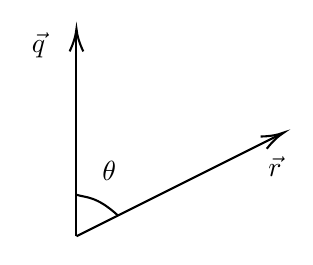
\begin{tikzpicture}[x=0.75pt,y=0.75pt,yscale=-1,xscale=1]
%uncomment if require: \path (0,300); %set diagram left start at 0, and has height of 300

%Straight Lines [id:da4402999370947803] 
\draw    (250,150) -- (250,52) ;
\draw [shift={(250,50)}, rotate = 90] [color={rgb, 255:red, 0; green, 0; blue, 0 }  ][line width=0.75]    (10.93,-3.29) .. controls (6.95,-1.4) and (3.31,-0.3) .. (0,0) .. controls (3.31,0.3) and (6.95,1.4) .. (10.93,3.29)   ;
%Straight Lines [id:da0037929251539179365] 
\draw    (250,150) -- (348.21,100.89) ;
\draw [shift={(350,100)}, rotate = 153.43] [color={rgb, 255:red, 0; green, 0; blue, 0 }  ][line width=0.75]    (10.93,-3.29) .. controls (6.95,-1.4) and (3.31,-0.3) .. (0,0) .. controls (3.31,0.3) and (6.95,1.4) .. (10.93,3.29)   ;
%Curve Lines [id:da06140636400336408] 
\draw    (250,130) .. controls (254.53,131.45) and (259.53,130.45) .. (270,140) ;

% Text Node
\draw (227,50.4) node [anchor=north west][inner sep=0.75pt]    {$\vec{q}$};
% Text Node
\draw (341,110.4) node [anchor=north west][inner sep=0.75pt]    {$\vec{r}$};
% Text Node
\draw (261,112.4) node [anchor=north west][inner sep=0.75pt]    {$\theta $};


\end{tikzpicture}